
%(BEGIN_QUESTION)
% Copyright 2011, Tony R. Kuphaldt, released under the Creative Commons Attribution License (v 1.0)
% This means you may do almost anything with this work of mine, so long as you give me proper credit

This PLC is supposed to control the position of a motor-actuated valve using a 4-20 mA analog signal.  However, there seems to be a problem: the valve remains in the fully-closed position even when it is supposed to open.  A voltmeter connected between terminals 3 and 2 initially registers 0 VDC, but then it registers 24 VDC when the conductor from cable 23 is disconnected from terminal 10:

$$\includegraphics[width=15.5cm]{i02393x01.eps}$$

Identify the likelihood of each specified fault for this circuit.  Consider each fault one at a time (i.e. no coincidental faults), determining whether or not each fault could independently account for {\it all} measurements and symptoms in this circuit.

% No blank lines allowed between lines of an \halign structure!
% I use comments (%) instead, so that TeX doesn't choke.

$$\vbox{\offinterlineskip
\halign{\strut
\vrule \quad\hfil # \ \hfil & 
\vrule \quad\hfil # \ \hfil & 
\vrule \quad\hfil # \ \hfil \vrule \cr
\noalign{\hrule}
%
% First row
{\bf Fault} & {\bf Possible} & {\bf Impossible} \cr
%
\noalign{\hrule}
%
% Another row
Cable 12 failed open &  &  \cr
%
\noalign{\hrule}
%
% Another row
Cable 15 failed open &  &  \cr
%
\noalign{\hrule}
%
% Another row
Cable 23 failed open &  &  \cr
%
\noalign{\hrule}
%
% Another row
Cable 41 failed open &  &  \cr
%
\noalign{\hrule}
%
% Another row
Cable 12 failed shorted &  &  \cr
%
\noalign{\hrule}
%
% Another row
Cable 15 failed shorted &  &  \cr
%
\noalign{\hrule}
%
% Another row
Cable 23 failed shorted &  &  \cr
%
\noalign{\hrule}
%
% Another row
Cable 41 failed shorted &  &  \cr
%
\noalign{\hrule}
} % End of \halign 
}$$ % End of \vbox

\underbar{file i02393}
%(END_QUESTION)





%(BEGIN_ANSWER)

% No blank lines allowed between lines of an \halign structure!
% I use comments (%) instead, so that TeX doesn't choke.

$$\vbox{\offinterlineskip
\halign{\strut
\vrule \quad\hfil # \ \hfil & 
\vrule \quad\hfil # \ \hfil & 
\vrule \quad\hfil # \ \hfil \vrule \cr
\noalign{\hrule}
%
% First row
{\bf Fault} & {\bf Possible} & {\bf Impossible} \cr
%
\noalign{\hrule}
%
% Another row
Cable 12 failed open &  & $\surd$ \cr
%
\noalign{\hrule}
%
% Another row
Cable 15 failed open &  & $\surd$ \cr
%
\noalign{\hrule}
%
% Another row
Cable 23 failed open &  & $\surd$ \cr
%
\noalign{\hrule}
%
% Another row
Cable 41 failed open &  & $\surd$ \cr
%
\noalign{\hrule}
%
% Another row
Cable 12 failed shorted &  & $\surd$ \cr
%
\noalign{\hrule}
%
% Another row
Cable 15 failed shorted &  & $\surd$ \cr
%
\noalign{\hrule}
%
% Another row
Cable 23 failed shorted &  & $\surd$ \cr
%
\noalign{\hrule}
%
% Another row
Cable 41 failed shorted & $\surd$ &  \cr
%
\noalign{\hrule}
} % End of \halign 
}$$ % End of \vbox

%(END_ANSWER)





%(BEGIN_NOTES)

{\bf This question is intended for exams only and not worksheets!}.

%(END_NOTES)


